\documentclass[12pt]{article}
\usepackage[english]{babel}
\usepackage[utf8x]{inputenc}
\usepackage[T1]{fontenc}
\usepackage{listings}
\usepackage{tikz}
\usepackage{/Users/songye03/Desktop/math_tex/style/quiver}
\usepackage{/Users/songye03/Desktop/math_tex/style/scribe}



\begin{document}
Songyu Ye

\today
\section{Theory}

The machinery developed in GKM is about the following setting. We have a torus acting 
on a manifold $X$ so that the following is true: \begin{enumerate}
    \item The $T$-action is equivariantly formal. There is a fibration $X \to ET\times_T X \xrightarrow{i} BT$
    and equivariantly formal is the condition that induced map $i^*$ is a surjection on cohomology.
    \item There are finitely many fixed points.
    \item There are finitely many $1$-dimensional orbits.
\end{enumerate}

There are many families of tori acting on spaces which are equivariantly formal. For example \begin{enumerate}
    \item smooth complex projective variety with a linear action of a torus.
    \item a variety whose ordinary cohomology vanishes in odd degree with any $T$-action.
    \item variety with $T$-invariant CW decomposition.
    \item compact symplectic manifold with a Hamiltonian $T$-action, where $T$ is the compact torus.
\end{enumerate}

In general, one seems to be able to relax these conditions sometimes. For example, in Knutson-Tao,
the authors only worry about the case where $X$ is a smooth projective variety, and $T$ acts on $Y$ algebraically with isolated fixed points.
In particular, Knutson-Tao worry about $X = \Gr(n,k)$ and $T$ is the $n$-dimensional torus acting on $\Gr(n,k)$ by scaling the coordinates.

\hfill



In this setting, one obtains a nice combinatorial description of the equivariant cohomology ring $H_T^*(X)$.
Under weaker conditions, Kirwan showed that $X^T\hookrightarrow X$ induces an injection on cohomology.

\begin{theorem}
    Let $T$ act on $X$ equivariantly formal and $X^T$ is finite. Then the inclusion $X^T\hookrightarrow X$ induces an injection on cohomology.
\end{theorem}

GKM showed that under the "GKM conditions" one has a nice description of the image of $H_T^*(X)$.
The main theorem: 

\begin{theorem}
    Suppose $T$ acts on $X$ with the GKM conditions. Then \begin{enumerate}
        \item The closure of each $1$-dimensional orbit $\cong \C\P^1$
        \item There are exactly 2 fixed points in each orbit closure, at the poles
        \item $T$ acts by rotation on each orbit
        \item each orbit has a subtorus $T'\subset T$ of comdimension $1$ which stabliizes the orbit pointwise.
    \end{enumerate}
\end{theorem}

This theorem allows us to make sense of the following combinatorial data, which we call the moment graph of $X$.
\begin{enumerate}
    \item The vertices are the fixed points of $X$.
    \item The edges are the $1$-dimensional orbits.
    \item The edges are labeled with the annihilator $\in \mf t^*$ of the tangent space of the stabliizer.
\end{enumerate}
\red{It is a fact that the moment graph is regular.}
\hfill

GKM further characterized the image of $H_T^*(X)$ in terms of the $1$-dimensional orbits. Let $O$ be a $1$-dimensional orbit and $N,S$ the north and south poles.
Let $f_N,f_S \in S(t^*)$ the corresponding classes in cohomology and $T'$ the stabilizer of $O$.
Then $f_N,f_S$ must agree on the tangent space $\mf t'$ of $T'$, i.e. $f_N - f_S$ is in the ideal generated by the annihilator of $\mf t'$.

\hfill

This is true because you look at the diagram $\set{O}\to\set{O\cup N},\set{O\cup S}\to\set{\bar O}$
 and the induced map on cohomology. The main content of their theorem is that this is in fact the full image.

 \begin{theorem}
    Let $T$ act on $X$ with the GKM conditions. Then \begin{align*}
        H_T^*(X) \cong\set{(f_1,\dots,f_n)\in S(t^*)^n\mid f_i - f_j \in \text{ideal generated by annihilator of }\mf t_i' \text{ for each $1$-diml orbit }O}
    \end{align*}
 \end{theorem}
 This is an isomorphism of rings, where the multiplication on the right hand side is multiplication of polynomials entrywise.

\section{Examples}

\begin{example}[nonexample]
Here is the standard example of non-equivariantly formal. 
Three copies of $\C\P^1$ in a triangle formation. The relevent torus $\C^*$
fixes the points of intersection and rotates each copy of $\C\P^1$ so that when acted on by $t\in\C^*$,
as $t\to 0$ the points of each $\C\P^1$ flow from the north pole to the south pole, 
and so that the north pole of each sphere is glued to the south pole of the next.
The problem is that $H^1_T(X)$ is nonzero.

\end{example}

\begin{example}
    Let $T^2$ act on $\C\P^2$ via $(t_1,t_2)\cdot [z_0:z_1:z_2] = [z_0:t_1z_1:t_2z_2]$.
    The fixed points are $[1:0:0],[0:1:0],[0:0:1]$ and the $1$-dimensional orbits are $[*:*:0], [*:0:*],[0:*:*]$.
    The moment graph is \begin{center}
        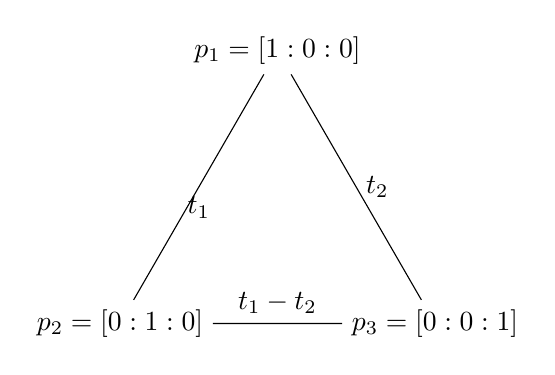
\begin{tikzpicture}
            \node (a) at (0,0) {$p_2 = [0:1:0]$};
            \node (b) at (4,0) {$p_3 = [0:0:1]$};
            \node (c) at (2,3.464) {$p_1 = [1:0:0]$};
            \draw (a) -- node[midway, above] {$t_1 - t_2$} (b) -- node[midway, right] {$t_2$} (c) -- node[midway, below] {$t_1$} (a);
        \end{tikzpicture}
    \end{center}
    Notice that the moment graph is the same as that of the nonexample, but this one is equivariantly formal.
    \red{What is the difference?}

    \hfill 

    Let's solve for generators and relations. Let $(f_1,f_2,f_3)$ be an element in cohomology.
    Then using the $12$ and the $13$ edge we can write $f_2 = f_1 + t_1g_1$ and $f_3 = f_1 + t_2g_2$.
    Then we impose the $23$ edge and get $\ideal{t_1 - t_2}\ni f_3 - f_2 = t_2g_2 - t_1g_1$, from 
    which we get $g_2 - g_1 \in \ideal{t_1 - t_2}$. So we can write $g_2 = g_1 + (t_2 - t_1)h$ \red{change signs here to agree with convention}.
    Plugging in, we see that \begin{align*}
        (f_1,f_2,f_3) = (f_1,f_1 + t_1g_1, f_1 + t_2g_1 + t_2(t_2 - t_1)h)
    \end{align*} where $f_1,g_1,h$ are arbitrary. So we see that $H_T^*(\C\P^2)$ is a free $S(t^*)$-module
    with additive basis \begin{align*}
        (1,1,1) \\ x = (0,t_1,t_2) \\ y = (0,0,t_2(t_2 - t_1))
    \end{align*} There is one generator in degree $2$ and one in degree $4$, which agrees with the Betti numbers of $\C\P^2$. There is one relation in equivariant cohomology \begin{align*}
        x^2 - t_1x = y
    \end{align*} which maps to the familiar relation in ordinary cohomology $x^2 = y$.
\end{example}

\begin{example}[full flag variety in $\C^3$ under the diagonal action of $(\C^*)^2$]
    The action is \begin{align*}
        (t_1,t_2)\cdot g = \begin{bmatrix}
            t_1 & 0 & 0 \\
            0 & 1 & 0 \\
            0 & 0 & t_2
        \end{bmatrix}g\begin{bmatrix}
            t_1^{-1} & 0 & 0 \\
            0 & 1 & 0 \\
            0 & 0 & t_2^{-1}
        \end{bmatrix}
    \end{align*} where $g$ is a matrix whose column span is a flag. The fixed points are the permutation matrices.
    The $1$-dimensional orbits are permutation matrices with a choice of box in the diagram on $\pi$. 
    The moment graph looks like 
    \begin{center}
    \includegraphics*[scale = .05]{/Users/songye03/Desktop/math_tex/img/IMG_1757.JPG}
    \end{center}
    One can play again the same divisibility game to get the generators. 
    They work out to be \begin{align*}
        (1,1,1,1,1,1) \\
        u_1 = (0,t_1,0,t_1,t_1-t_2,t_1 - t_2) \\ 
        u_2 = (0,0,t_2,-t_1 + t_2,t_2,-t_1 + t_2) \\ 
        v_1 = (0,0,0,t_1(t_1- t_2),0,t_1(t_1- t_2)) \\ 
        v_2 = (0,0,0,0,t_2(t_1 - t_2),t_2(t_1 - t_2)) \\ 
        w = (0,0,0,0,0,t_1t_2(t_1-t_2))
    \end{align*} \red{they should correspond to permutations but I'm not sure how. One way is 
    to associate the generator to where it first appears in the divisibility game, but does that even make sense?}
    The (partial list of) relations are \begin{align*}
        u_1^2 - t_1u_1 = -v_2 \\ 
        u_2^2 + t_2u_2 = v_1 \\ 
        u_1u_2 = -v_1 + v_2
    \end{align*} \red{there should be another relation involving $w$ but I couldn't figure it out. Also what should $u_1^3$ be?}
    Also this fails the arrow rule terribly.
\end{example}

\begin{example}[Grassmannian $\Gr(4,2)$ under Plucker embedding]
    The hypersurface $x_1y_1 + x_2y_2 + x_3y_3 = 0$ has a $T^3$-action given by
    \begin{align*}
        (t_1,1,1)\cdot (x_1,x_2,x_3,y_1,y_2,y_3) &= (t_1x_1,t_1x_2,t_1x_3,y_1,y_2,y_3) \\ 
        (1,t_2,1)\cdot (x_1,x_2,x_3,y_1,y_2,y_3) &= (t_2x_1,t_2x_2,x_3,y_1,y_2,t_2y_3) \\ 
        (1,1,t_3)\cdot (x_1,x_2,x_3,y_1,y_2,y_3) &= (t_3x_1,x_2,t_3x_3,y_1,t_3y_2,y_3)
    \end{align*}
    There are $6$ fixed points corresponding to the coordinates. There are $12$ 1-dimensional orbits corresponding to 
    the $\binom{6}{2} - 3$ pairs of coordinates, excluding the ones $(x_i,y_i)$. The moment graph looks like 
    \begin{center}
        \includegraphics*[scale = .5]{/Users/songye03/Desktop/math_tex/img/Screenshot 2024-01-17 at 2.50.46 PM.png}
    \end{center}
    Playing the same divisibility game, one obtains generators \begin{align*}
        & (1,1,1,1,1,1) \\
        u_1 &= (0,t_3,t_2,t_3-t_1,t_2-t_1,t_3 + t_2 - t_1) \\ 
        v_1 &= (0,0,t_2(t_2-t_3),0,(t_2-t_1)(t_2-t_3),t_2(t_2-t_1)) \\
        v_2 &= (0,0,0,t_1(t_1-t_3),t_1(t_1-t_2),(t_1-t_3)(t_1-t_2)) \\
        w_1 &= (0,0,0,0,t_1(t_1-t_2)(t_2-t_3),t_2(t_1-t_2)(t_1-t_3)) \\
        x_1 &= (0,0,0,0,0,t_2t_3(t_1-t_2)(t_1-t_3))
    \end{align*} I have put an implicit numbering of the vertices, it is $x_1,x_2,x_3,y_3,y_2,y_1$. \red{what should it be?}
\end{example}

\begin{remark}
    What is the point of studying these examples?
    \begin{enumerate}
        \item Sometimes one can read off the generators of equivariant cohomology from the moment graph, by looking at the way the arrows point.
        \item The arrow rule works for $\C\P^2$ but it does not work for the flag variety nor the Grassmannian. It seems to work for all of Tara's examples, namely $G_2/P$, the loop group, and the homogenous space of type $A_1^{(4)}$.
        \item The relations are not clear at all.
        \item Computations are aided by introducing a partial order on the vertices of the moment graph. 
    \end{enumerate}
\end{remark}



\section{Grassmannians}
In this section we will consider the ordinary and equivariant cohomology of Grassmannians.
Let $\Gr(n,k)$ denote the Grassmannian of $k$-dimensional subspaces of $\C^n$.
For each $\lambda \in \binom{[n]}{k}$, there is a Schubert cycle \begin{align*}
    X_\lambda = \set{V\in\Gr(n,k)\st \dim(V\cap F_i)\geq \dim(\C^\lambda \cap F_i) \text{ for all $i$}}
\end{align*} where $F_i$ is antistandard $i$-plane. The Poincare duals of Schubert cycles are known as Schur polynomials and they form an additive $\Z$-basis of $H^*(\Gr(n,k))$.
The $x_i$ denote the Chern classes of the tautological bundle $\gamma_k$ over $\Gr(n,k)$.

Schubert calculus is concerned about multiplication in the cohomology ring of Grassmannians. In 
particular there are structure constants \begin{align*}
    x_\lambda x_\mu = \sum_\nu c_{\lambda\mu}^\nu x_\nu
\end{align*} where $c_{\lambda\mu}^\nu$ are the Littlewood-Richardson coefficients. These guys can 
be computed in many ways, Knutson and Tao like puzzles.

\hfill

Now let's consider the equivariant cohomology of Grassmannians. Let $T^n$ act on $\Gr(n,k)$ diagonally.
The fixed points are the $\binom{n}{k}$ standard $k$-planes. The $1$-dimensional orbits are indexed by transpositions.

\hfill

There is a partial order on $\lambda \in \binom{[n]}{k}$ given by $\lambda \leq \mu$ if 
$\sum_{1\leq i\leq j} \lambda_i \leq \sum_{1\leq i\leq j} \mu_i$ for all $1\leq j\leq n$. 
Let $\alpha$ be an element of $H^*_T(\Gr(n,k))$. Then we say that $\alpha$ is a Schubert class corresponding
to $\lambda$ if $\alpha$ is supported above $\lambda$, $\alpha\vert_\lambda = \prod_{(i,j)\text{ inversion}}y_j - y_i$, and 
$\alpha\vert_\mu$ is homogenous of degree $l(\lambda)$ for all $\mu$.

\hfill 

Schubert classes exist uniquely for each $\lambda$. They form an additive basis of $H^*_T(\Gr(n,k))$ for geometric reasons.
The point is that if $Y$ is a smooth projective variety and $T$ acts on $Y$ algebraically with isolated fixed points, then 
$Y$ has a cell decomposition by complex cells $X_f$ corresponding to the $T$-fixed points. The equivariant cohomology of $Y$ is
the free $S(t^*)$-module generated by the cells.

\hfill

The Schubert cycles $X_\lambda$ are oriented and $T$ invariant, so they induce equivariant cohomology classes $[X_\lambda]_T$.
In general this is true for any $T$-invariant oriented cycle in a compact oriented manifold. 
These cycles are the closures of a cell decomposition of $\Gr(n,k)$ into complex cells.

\hfill

Bump describes another way of producing the CW decomposition. For $w\in W$ the Weyl group, the double coset $BwP/P$ is homeomorphic 
to $\C^{\ell(w)}$ and the closure of $BwP/P$ is a cell. The closure of $BwB/B$ is the Schubert variety $X_w$, and the classes of 
the closures form an additive basis for $H^*_T(\Gr(n,k))$.

\hfill

Here are the six Schubert classes in $H^*_T(\Gr(4,2))$:
\begin{center}
    \includegraphics*[scale = .25]{/Users/songye03/Desktop/math_tex/img/Screenshot 2024-01-18 at 4.23.13 PM.png}
\end{center}

Each generator correpsonds to the choice of $\binom{4}{2}$ string of $0$'s and $1$'s. In particular, we know what the value of the generator is on the fixed point 
to which it corresponds. As for the other fixed points, one can use transpositions and swap the variables accordingly. \red{This works everytime except for in degree $1$. 
It is also not clear how the module generators correpsond to partitions which fit inside a $2\times 2$ box. It is also not clear what the forgetful map to ordinary cohomology does. The arrow rule also does not work.}

\begin{remark}
    There is a note in Knutson-Tao that the data of these lists of polynomials is secretly the same as the data of one big polynomial in many variables.
\end{remark}
\section{Flag varieties}
In this section we will consider the ordinary and equivariant cohomology of flag varieties.

\hfill

For reasons which are not clear to me, the story of ordinary cohomology of the flag variety is quite similar to that of Grassmannians.
Let $X$ be the full flag variety in $\C^n$. There are Schubert varieties $X_w$ for each $w\in S_n$ defined by the following recipe.
If $w = 526134$ then $X_w$ is the closure of the open Schubert variety $X_w^{o} = BwB/B$ which is all flags which look like \begin{align*}
    \begin{bmatrix}
        * & * & * & * & 1 & 0 \\
        * & 1 & 0 & 0 & 0 & 0 \\
        * & 0 & * & * & 0 & 1 \\
        1 & 0 & 0 & 0 & 0 & 0 \\
        0 & 0 & 1 & 0 & 0 & 0 \\
        0 & 0 & 0 & 1 & 0 & 0
    \end{bmatrix}
\end{align*}
The classes of the Schubert varieties form an additive basis of $H^*(X)$. On $X$, one has a tautological flag of subbundles 
\begin{align*}
    0 = F_0 \subset F_1 \subset \dots \subset F_n = \C^n
\end{align*} and Chern classes $x_i = -c_1(\gamma_i)$ where $\gamma_i = F_i/F_{i-1}$. 
Since the elementary symmetric polynomials are the Chern classes of the trivial bundle, it follows that $e_i(x) = 0$ in $H^*(X)$.

Then \begin{align*}
    H^*(X) \cong \Z[x_1,\dots,x_n]/\ideal{e_1(x),\dots,e_n(x)}
\end{align*} \red{One sees this geometrically using the construction of $X$ as a sequence of projective bundles.}

\hfill 

BGG and Demazure solved how to write the classes of Schubert varieties in terms of the Chern classes. The answer is Schubert polynomials.
\begin{align*}
    [X_w] = \partial_{w^{-1}}(x_1^{n-1}\cdot \dots \cdot x_{n-1}^1)
\end{align*}

\hfill

I didn't find any reference for the equivariant cohomology of flag varieties. There is a note on the bottom of Knutson-Tao
that says arguments for the Grassmannian should work for flag varieties, but Knutson-Tao couldn't find it. \red{What about now?}

\red{How does Schubert calculus work in equivariant cohomology of flag varieties?}

\hfill

\red{In the examples concerning flags in $\C^3$ and $\Gr(4,2)$ the torus action is different than the torus action that Knutson-Tao consider.
Should the general theory give insight into that torus action?}

\subsection{Cell structure on the flag variety}
Recall the Bruhat decomposition for $\GL(n,\C)$. Let $T$ be the diagonal matrices and $B$ be the standard Borel of upper triangular matrices. 
Consider the Weyl group $W = N(T)/T = S_n$. \begin{theorem}
    One can write $\GL(n,\C)$ as a disjoint union of double cosets \begin{align*}
        \GL(n,\C) = \bigsqcup_{w\in W} BwB
\end{align*}
\end{theorem}
For $\GL(n,\C)$, this decomposition actually just follows from row reduction. The $B\times B$ orbits
correspond to upward row operations and rightward column operations. 

\begin{example}
    The matrix \begin{align*}
        \begin{bmatrix}
            7 & 1 & 2 \\
            1 & 1 & -2 \\
            2 & 8 & 4
        \end{bmatrix}
    \end{align*} I can clear the first column using upward row operations, and then I can clear the third row using rightward column operations.
    \begin{align*}
        \begin{bmatrix}
            0 & * & * \\
            0 & * & * \\
            1 & 0 & 0 
        \end{bmatrix}
    \end{align*} and then I can continue. For generic matrix,
    doing this will end me up at the longest permutation $321$. This is called the \textbf{big cell} and it is 
    dense in $\GL(n,\C)$. If the bottom left entry were $0$, then I could not do this, but instead I would 
    go up the first column looking for a nonzero entry, clear everything above it and to the right of it, and continue.
\end{example}

The Bruhat stratification of $\GL(n,\C)$ descends to a cell structure of the flag variety $X = \GL(n,\C)/B$.
In particular each orbit $BwB$ descends to an affine space $X^w_o = BwB/B$, which Allen denotes the \textbf{opposite Schubert cell}.
The image of the $B_{-}wB$ orbit is the Schubert cell $X_w^o = B_-wB/B$ and its closure is called a \textbf{Schubert variety} $X_w$.
A key fact is that each of the open opposite Schubert cells is isomorphic to an affine space of dimension $\ell(w)$.

\begin{example}
    Consider $w = 132$. Then we are thinking about the $B\times B$ orbits of the matrix \begin{align*}
        \begin{bmatrix}
            1 & 0 & 0 \\
            0 & 0 & 1 \\
            0 & 1 & 0
        \end{bmatrix} 
    \end{align*} We are using the row convention for writing permutation matrices.
    The $B\times B$ orbit looks like \begin{align*}
        \begin{bmatrix}
            * & * & * \\
            0 & * & * \\
            0 & * & *
        \end{bmatrix}
    \end{align*} where the $*$ are almost arbitrary, they are subject to some nondegeracy conditions (for example the 
    $1,1$ star cannot be zero and so on). When I mod out by $B$, I am looking at the successive column spans and every such
    flag can be written uniquely by a matrix \begin{align*}
        \begin{bmatrix}
            1 & 0 & 0 \\
            0 & * & 1 \\
            0 & 1 & 0
        \end{bmatrix} 
    \end{align*} which is indeed of dimension $1$.
    
    The $B_-\times B$ orbit looks like \begin{align*}
        \begin{bmatrix}
            * & * & * \\
            * & 0 & * \\
            * & * & *
        \end{bmatrix} 
    \end{align*} and once I look up to column span they look like \red{?? maybe} \begin{align*}
        \begin{bmatrix}
            1 & 0 & 0 \\
            * & 0 & 1 \\
            * & 1 & 0
        \end{bmatrix}
    \end{align*}

\end{example}
\hfill

The key fact we use is that the each Schubert variety is the closure of an open subvariety (a Schubert cell) which is
isomorphic to an affine space, and the union of the Schubert cells in the closure of a Schubert cell is the corresponding Schubert variety.

\hfill

This allows us to conclude that the Schubert classes give an addivitive basis of the cohomology of the flag variety (and Grassmannian)
\section{Loop groups}

Consider $\Omega G = LG/G$ where $G$ is a Lie group. The loop group $LG$ is the space of maps $S^1\to G$ of Sobolev class $H^1$.
$\Omega G$ is a homogenous space (smooth manifold endowed with a transitive smooth action by $LG$) for $LG$.
There is a torus action on $\Omega G$. The maximal torus of $G$ is a subgroup of $LG$ and acts on the left on $\Omega G$ by \begin{align*}
    t\gamma(\theta) = t\gamma(\theta)t^{-1}
\end{align*}
There is also a rotation action by $S^1$ \begin{align*}
    e^{is}\cdot \gamma(\theta) = \gamma(\theta + s)\gamma(s)^{-1}
\end{align*} and these actions commute, giving us $T\times S^1$ action on $\Omega G$.
The action is Hamiltonian with respect to the Kahler structure on $\Omega G$. This tells us that the action is equivariantly formal.

\hfill

Now consider the case $G = SU(2)$. We study this because $SU(2)$ is compact and simply connected, and it is the simplest such example.
In this case, there is a generator in each even degree, and the ring is generated by the one in degree two.

\hfill

The moment graph and the first couple of generators look like the following: 
\begin{center}
    \includegraphics*[scale = .25]{/Users/songye03/Desktop/math_tex/img/Screenshot 2024-01-18 at 5.48.26 PM.png}
    \includegraphics*[scale = .25]{/Users/songye03/Desktop/math_tex/img/Screenshot 2024-01-18 at 5.47.39 PM.png}
\end{center}

\red{This group is infinite dimensional, the fixed point set is still isolated but now
it is infinite, and there are infinitely many 1-dimensional orbits. How does one identify the fixed points of the
action, and why are they indexed by integer points on a parabola? Why are the edges indexed by critical values of the moment graph? Are they the same thing as the $1$-dimensional orbits?
Why does the divisibility game still work?}

\section{Wonderful compactifications}
Let $G$ be a complex connected semisimple group with trivial center, and let $\tilde G$ be
the universal cover of $G$. Let $V$ be an irreducible representation of $\tilde G$ 
of highest weight $\lambda$. We ask that $\lambda$ is regular, which means that $\langle \lambda, \alpha\rangle > 0$ for every
positive coroot $\alpha$. The regular weights are those which lie in the interior of the Weyl chamber.

The representation map $\tilde G\to \End(V)\backslash 0$ 
descends to a map $G \to \P(\End(V))$, which is $G\times G$-equivariant. $G\times G$ acts on $G$ via \begin{align*}
    (g_1,g_2)\cdot g = g_1gg_2^{-1}
\end{align*} and $\tilde G\times \tilde G$ acts on $\P(\End(V))$ via \begin{align*}
    (g_1,g_2)\cdot [v] = [g_1vg_2^{-1}]
\end{align*} and this descends to a $G\times G$ action on $\P(\End(V))$. 

\begin{definition}
    The wonderful compactification of $G$ is the closure of the image of $G$ in $\P(\End(V))$. \red{It has a $G\times G$ action. Why? It is only clear before
    we take closures.}
\end{definition} 

\begin{example}
    $G = PGL(2)$ and $\tilde G = \SL(2,\C)$. Then every nonzero dominant weight is regular and so we can
    take $V = \C^2$ the standard representation. Then the embedding $\psi:G\to\P(M(2,2))$
    is the embedding with image \begin{align*}
        \set{\begin{bmatrix}
            a & b \\
            c & d
            \end{bmatrix}\st ad - bc = 1} 
    \end{align*} and the closure of this is all of $\P(M(2,2))$. There is a $G\times G$ action on this space 
    which is just standard matrix multiplication.
\end{example}

\begin{remark}
    In general the wonderful compactification of $PGL(n)$ is not simply projective space.
\end{remark}

So we have a $T\times T$ action on the wonderful compactification. Allen suggested applying the GKM machinery in this case.

\subsection{Geometry}
Given $G$ acting on a variety $V$, a wonderful compactification of $V$ is a $G$-equivariant compactification so that each orbit closure is smooth.
Wonderful varities first appeared in the work of De Concini and Procesi, who constructed them for symmetric homogenous spaces $G/H$ where $H = G^\sigma$ is the fixed point set of an involution $\sigma$ of $G$.
The properties were so nice that people took them for axioms.

\begin{definition}
    Let $X$ be a $G$-variety. Then $X$ is wonderful if \begin{enumerate}
        \item $X$ is smooth and complete
        \item $X$ has an open $G$-orbit $X_G^o$ and the complement $X\setminus X_G^o$ is a union of smooth $G$-invariant divisors $D_1,\dots,D_r$ who have normal crossings and nonempty intersections.
        $r$ is called the rank of $X$.
        \item For all $x,y\in X$ we have \begin{align*}
            Gx = Gy \implies \set{i\st x\in D_i} = \set{j\st y\in D_i}
        \end{align*}
    \end{enumerate}
\end{definition}
On a wonderful variety, the $G$-orbits are exactly the sets (indexed by $I\subset\set{1,\dots,r}$)
\begin{align*}
    \bigcap_{i\in I}D_i \setminus \bigcup_{j\notin I}D_j
\end{align*} Thus a wonderful variety has exactly $2^r$ orbits, exactly one of which is closed. Any wonderful variety is spherical (Luna).

\begin{example}
    The canonical example of De Concini and Procesi are symmetric homogenous spaces $G/H$ where $H = G^\sigma$ is the fixed point set of an involution $\sigma$ of $G$.
    In this case we have a canonical wonderful compactification $G/H \to X$ with an action of $G$ so that \begin{enumerate}
        \item $X$ has an open orbit $\cong G/H$
        \item $X$ is smooth and has finitely many $G$-orbits
        \item Orbit closures are smooth 
        \item There is a $1-1$ correspondence with sets of orbit closures $S_J$ and subsets of a set $J \subset I_l$ with $l$ elements.
        \item $J \subset I_l$ then $S_I \cap S_J = S_{I\cup J}$ and $\codim S_I = \abs{I}$
        \item Each $S_I$ is the transversal complete intersection of the $S_{\set{i}}$
        \item Each $S_I$ we have $G$ equivariant fibration $\pi_I:S_I\to G/P_I$ where $P_I$ is the parabolic subgroup of $G$ with semisimple Levi factor $L$, $\sigma$ stable, 
        and the fiber of $\pi_I$ is the canonical wonderful compactification of $L$.s
    \end{enumerate}

\end{example}

\begin{example}
    The symmetric homogemous spaces $G\times G/G$ for $G$ semisimple adjoint (ex. $G = \P\GL(n)$) admit a wonderful compactification.
\end{example}

\begin{example}
    The wonderful compactification of $G = PGL(2)$ is $\P(M(2,2))$. This is for the following reason. Let $\tilde G = \SL(2)$ the universal cover.
    Then all nonzero weights are regular and we can take $V = \C^2$ the standard representation in the constructed above. Then the embedding $\psi:G\to\P(M(2,2))$
    has image \begin{align*}
        \psi(G) = \set{\begin{bmatrix}
            a & b \\
            c & d
            \end{bmatrix}\st ad - bc = 1
        }
    \end{align*}
    The closure of this is all of $\P(M(2,2))$. The boundary of $X$ is \begin{align*}
        \partial X = \set{\begin{bmatrix}
            a & b \\
            c & d
            \end{bmatrix}\st ad - bc = 0} \cong \P^1\times \P^1
    \end{align*}
\end{example}
\begin{remark}
    In general the wonderful compactification of $PGL(n)$ is not simply projective space, for the reason that the standard represetnation of $\SL(n)$ is not regular.
\end{remark}

\begin{example}
    For $\SL(2)$ the wonderful compactification is \begin{align*}
        X = \set{ad-bc = t^2}\subset \P(M(2,2)\oplus \C)
    \end{align*}
\end{example}

\begin{remark}
    \begin{enumerate}
        \item What are the open $G\times G$ orbits?
        \item What are the prime divisors?
        \item Do the computation for $\P\SL(n)$
    \end{enumerate}
\end{remark}
\subsection{Cohomology}
(Fulton) Whenever a variety has a filtration by closed subspaces so that successive differences are disjoint unions of spaces each isomorphic to affine space, the classes of the closures of these varieties
form an additive basis of the cohomology ring. \red{is this the case for our wonderful compactification?}

Recall that in the story of the flag variety $X = G/B$, $X$ is covered by open affine cells $X_w^o = BwB/B$. The closures are
Schubert varities and they have the property that they are the unions of Schubert cells \begin{align*}
    \overline{X_w^o} = \bigcup_{v\leq w} X_v^o
\end{align*}
This decomposition helped us understand the cohomology of the flag variety. Intimately related to this idea of using pieces of 
stratification to compute cohomology are the results of Bialynick and Birula.

\begin{theorem}
    Let $Z$ be a $\C^*$-variety with finitely many fixed points $z_1,\dots,z_r$. Let \begin{align*}
        C_i = \set{z\in Z\st \lim_{t\to 0} t\cdot z \in z_i}
    \end{align*} Then \begin{enumerate}
        \item Z = $\bigsqcup_{i=1}^r C_i$
        \item $C_i\cong T^+_{z_i}Z$ the positive tangent space at $z_i$ (positive weights). In particular each $C_i$ is isomorphic to affine space.
        \item $C_i$ is locally closed in $Z$.
    \end{enumerate} As a result $H_*Z$ has a basis given by the cycles corresponding to $\overline{C_i}$.
\end{theorem}

\begin{example}
    Consider $X = \C\P^n$ with the $\C^*$ action \begin{align*}
        t\cdot [z_0:\dots:z_n] = [t^n z_0:\dots:t^0z_n]
    \end{align*} The fixed points are the coordinate vectors and the cell decomposition is the standard one.
\end{example}

\begin{remark}
    \begin{enumerate}
        \item Does BB say aanything about ring multiplication?
        \item Does BB have equivariant story?
        \item Does BB apply to $Fl(n),\Gr(n,k)$?
        \item Does BB say anything about $\inf$-dimensional varieties or in the case of $\inf$-many orbits?
    \end{enumerate}
\end{remark}

Allen wrote on Stack Exchange in 2010 about how to apply $BB$ to the flag variety to obtain the Schubert stratification by open affines.
\begin{align*}
    Y = \GL_n/B \hookrightarrow \prod_{k=1}^n\Gr(n,k)\hookrightarrow \prod_{k=1}^n \P(\bigwedge^k\C^n)
\end{align*} the second map is the Plucker embedding. Now let $\C^*$ act on $X$ by \begin{align*}
    t\cdot (V_1,\dots,V_n) = (tV_1,\dots,t^nV_n)
\end{align*} Part of the $BB$ theorem is that if $Y\subset X$ is $\C^*$-invariant then $Y$ has a similar decomposition and $Y_p = X_p\cap Y$.
Then we see that $X_p$ is indexed by lists of subsets and $Y_p$ is indexed by lists of increasing lists of subsets, i.e. permutations.


\begin{thebibliography}{9}

\end{thebibliography}
\end{document}